\documentclass{beamer}

\usepackage[italian]{babel}
\usepackage{graphicx}
\usepackage{url}
\usepackage{soul}
\usepackage{tikz}
\usepackage{listings}
\usepackage{xcolor}
\usepackage{algorithm}
\usepackage{multicol}
\usepackage{textcomp}
\usepackage[noend]{algpseudocode}

\setbeamertemplate{navigation symbols}{}
\usetheme{default}
\usecolortheme{Nord}

% titolo, ...
\title{CoderFarm - Corso avanzato}
\subtitle{Lezione 1}
\author{Lorenzo Ferrari, Davide Bartoli}
\date{\today}

\begin{document}

\begin{frame}
    \titlepage
\end{frame}

\begin{frame}{Contenuti}
    \tableofcontents
\end{frame}

\section{Ricorsione}
\begin{frame}{Ricorsione}{Introduzione}
    Spesso risulta comodo formulare un problema in maniera ricorsiva, ossia in funzione di istanze pi\`u piccole dello stesso problema.
    \pause
    Prendiamo per esempio i numeri di Fibonacci
    \[
        F_n =
        \begin{cases}
            1 \quad & \text{per } 0 \leq n \leq 1 \\
            F_{n-1} + F_{n-2} & \text{per } n \geq 2
        \end{cases}
    \]
    \pause
    o il fattoriale
    \[
        n! =
        \begin{cases}
            1 & \text{per } n = 0 \\
            n \cdot (n-1)! & \text{per } n \geq 1
        \end{cases}
    \]
    \pause
    Queste definizioni possono essere scritte in C++ usando delle \textbf{funzioni ricorsive}.
\end{frame}

\begin{frame}{Funzioni ricorsive}{}
    Una funzione ricorsiva \`e una funzione che richiama se stessa.\\
    \pause 
    Deve sempre essere definita una condizione di terminazione, ossia un caso base in cui la funzione non richiama se stessa,
    altrimenti si entra in un ciclo infinito.
\end{frame}

\begin{frame}
    \makebox[\textwidth]{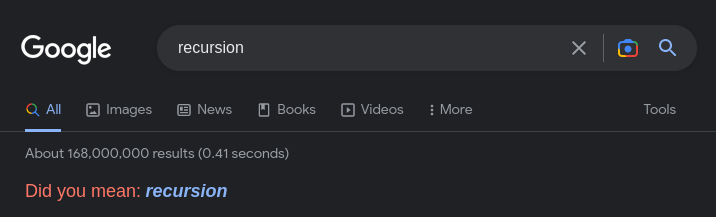
\includegraphics[scale=.30]{./img/recursion_google.png}}
    \vfill
    \pause
    \makebox[\textwidth]{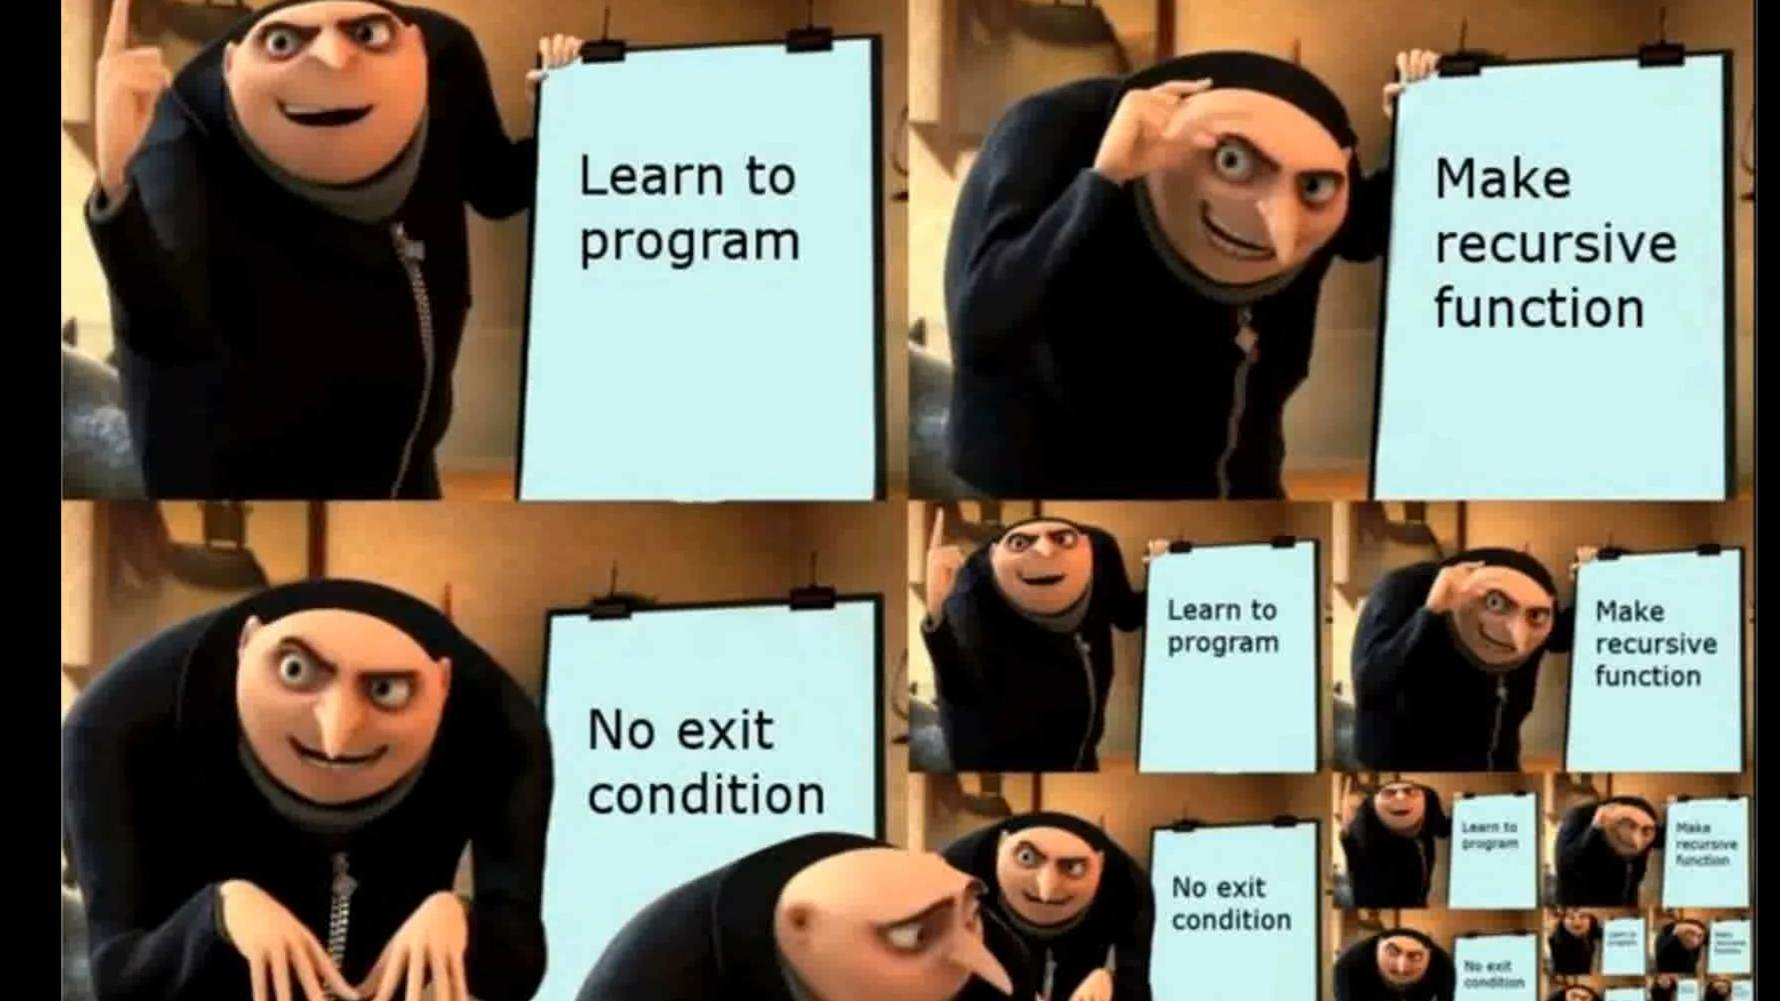
\includegraphics[scale=.15]{./img/no_exit_condition.jpg}}
\end{frame}

\begin{frame}{Ricorsione}{Funzioni ricorsive}
    \makebox[\textwidth]{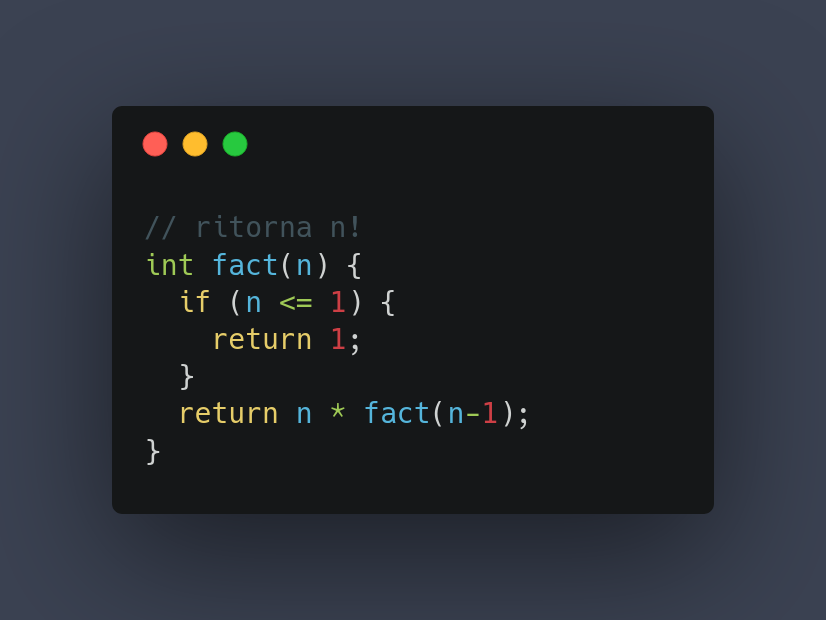
\includegraphics[scale=.30]{./img/fattoriale.png}}
\end{frame}

\begin{frame}{Ricorsione}{Funzioni ricorsive}
    \makebox[\textwidth]{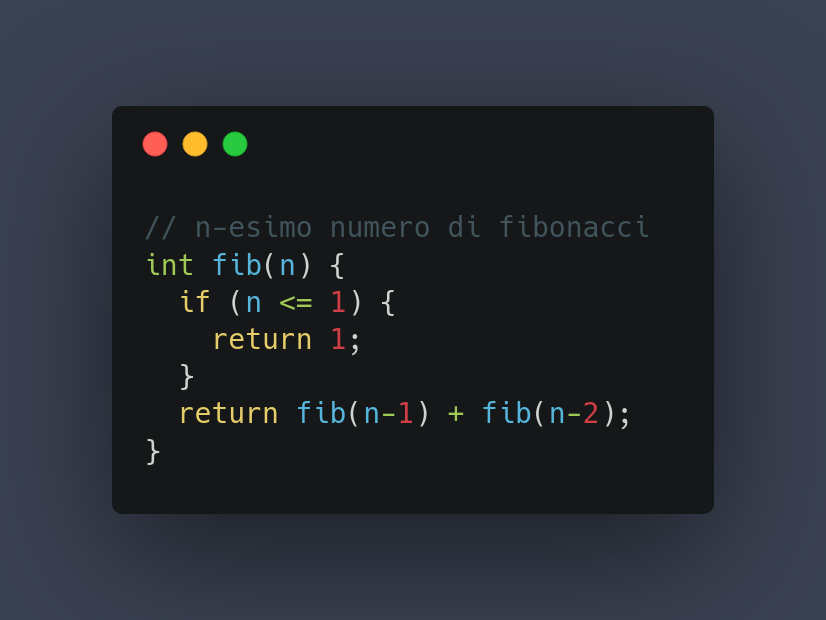
\includegraphics[scale=.30]{./img/fibonacci.png}}
\end{frame}

\begin{frame}{Albero di ricorsione}{}
    \begin{block}{}
        Le chiamate alla funzione ricorsiva \texttt{fib} formano un albero detto \textbf{albero di ricorsione}. \\
        Nel caso del fattoriale, l'albero \`e una linea con $N$ nodi.
    \end{block}
    \pause
    \vfill
    \makebox[\textwidth]{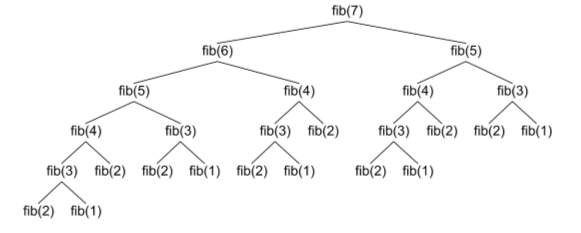
\includegraphics[scale=.70]{./img/fibonacci_tree.png}}
    \vfill
\end{frame}

\begin{frame}{Problema di riscaldamento}{Generare tutte le soluzioni}
    \begin{exampleblock}{Piastrelle}
        Vuoi piastrellare un corridoio di dimensione $1 \times N$ e hai a disposizione solo piastrelle di 
        dimensioni $1 \times 1$ e $1 \times 2$. Stampa tutte le possibili piastrellature di lunghezza $N$.
    \end{exampleblock}
    \pause
    \vfill
    \makebox[\textwidth]{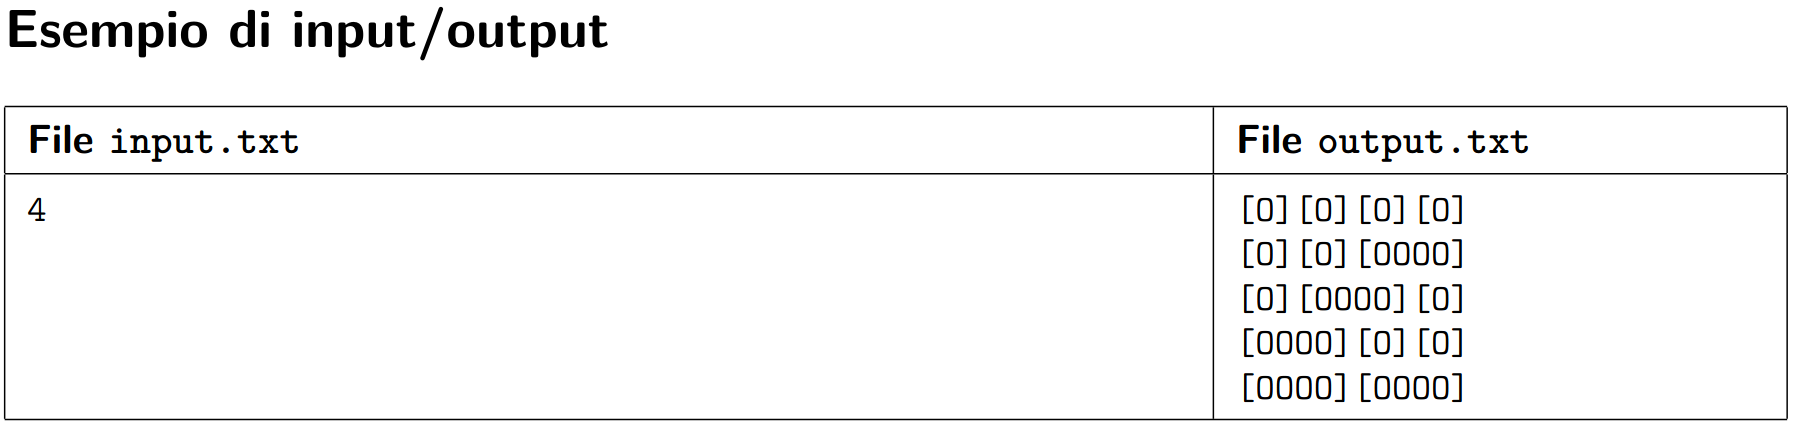
\includegraphics[scale=.15]{./img/piastrelle_esempi.png}}
    \vfill
    \small{\underline{\url{https://training.olinfo.it/\#/task/piastrelle/statement}}}
\end{frame}

\begin{frame}{Implementazione}{}
    \makebox[\textwidth]{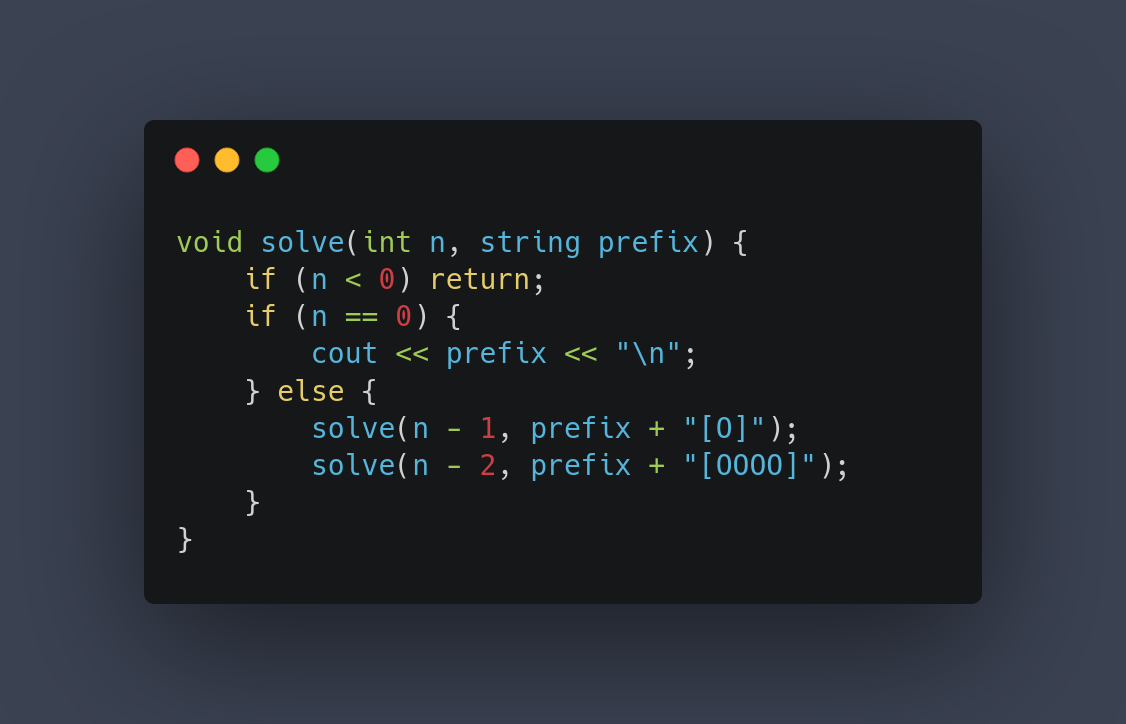
\includegraphics[scale=.30]{./img/piastrelle.png}}
\end{frame}

\section{Ricerca completa}

\begin{frame}{Ricerca completa}
    \begin{block}{}
        Quando esploriamo tutto lo spazio delle soluzioni eseguiamo una \textbf{ricerca completa}.
        \pause
        \bigbreak
        Spesso \`e possibile \emph{tagliare} alcuni rami dell'albero di ricorsione sapendo che la risposta migliore 
        non si trova in quel sottoalbero, e in alcuni casi possiamo evitare di ricalcolare pi\`u volte la stessa cosa. \\
    \end{block}
    La ricerca completa spesso permette di risolvere i primi subtask di un problema!
    \vfill
    \small{\underline{\url{https://training.olinfo.it/\#/task/ois_solitario/statement}}}
\end{frame}

%
% Pausa ?
%

\section{Programmazione Dinamica}
\begin{frame}{Programmazione Dinamica}{Fibonacci}
    Torniamo un momento al calcolo dell'$n$-esimo numero di Fibonacci. Quante chiamate stiamo facendo?
    \pause
    \begin{itemize}
        \item un numero esponenziale (in questo caso $O(\phi ^ n)$, dove $\phi = 1.618\dots$), decisamente troppe...
    \end{itemize}
    Si pu\`o fare meglio di cos\`i?
    \pause
    \begin{itemize}
        \item stiamo calcolando pi\`u volte $F_n$ per uno stesso $n$, che \`e molto inefficente
        \item in totale dobbiamo calcolare solo $O(n)$ valori, i numeri $F_0, F_1, \dots, F_n$. Possiamo quindi 
        salvarci i valori calcolati e riutilizzarli all'occorrenza. La complessit\`a \`e quindi $O(n)$.
        \item Questa tecnica di \textbf{memorizzazione} \`e alla base della \textbf{programmazione dinamica}.
    \end{itemize}
\end{frame}

\begin{frame}{Programmazione Dinamica}{Memoization}
    \makebox[\textwidth]{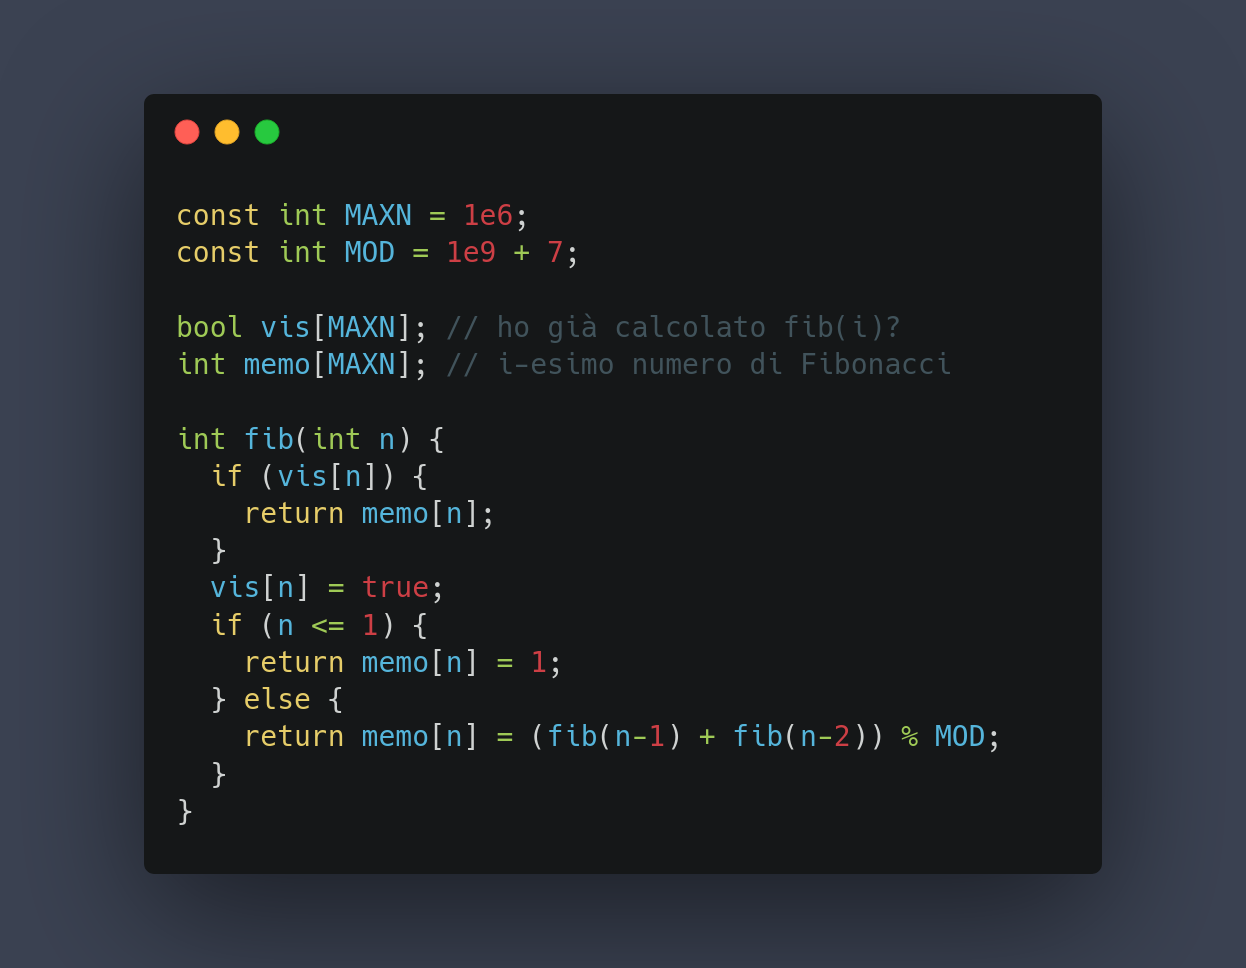
\includegraphics[scale=.25]{./img/fibonacci_memo.png}}
\end{frame}
%
\begin{frame}{Programmazione Dinamica}{DP Iterativa}
    \makebox[\textwidth]{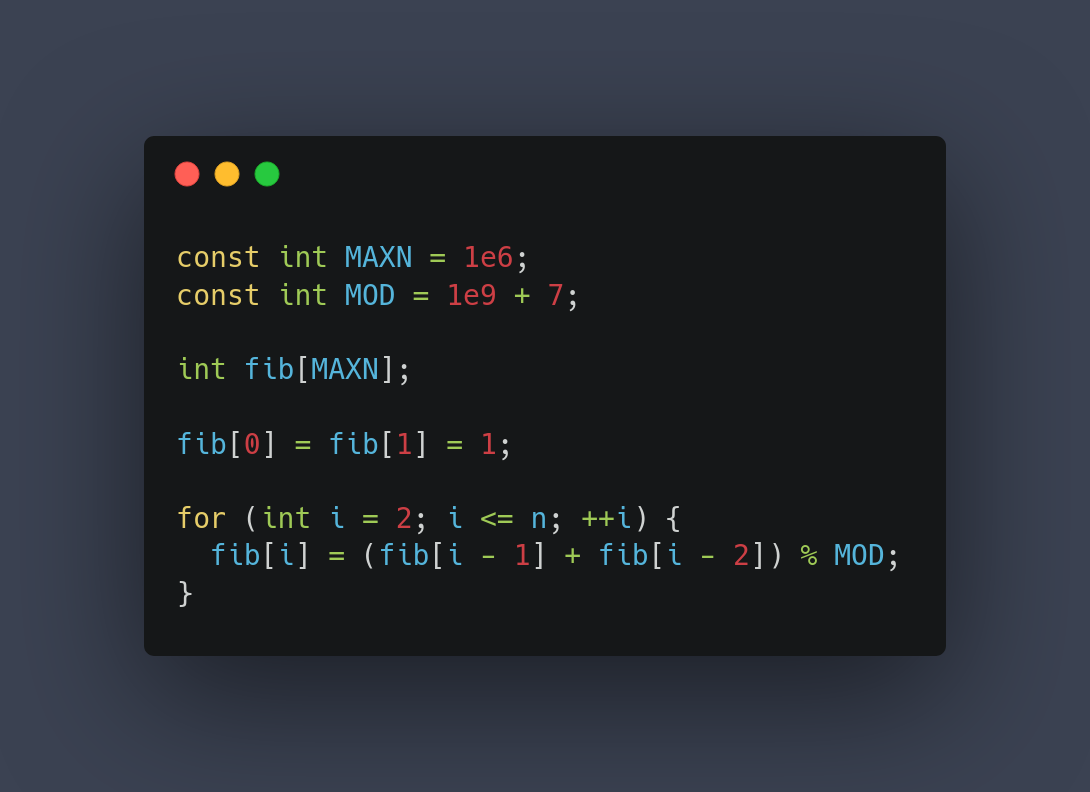
\includegraphics[scale=.30]{./img/fibonacci_iter.png}}
\end{frame}
%
\begin{frame}{Programmazione Dinamica}
    La programmazione dinamica permette di risolvere problemi apparentemente complessi in modo efficiente grazie alla memorizzazione dei risultati parziali. \\
    \vfill
    Pu\`o essere applicata a problemi che possono essere decomposti in sotto-problemi \textbf{indipendenti}.\\
    \vfill
    \pause
    \`E caratterizzata da:
    \begin{itemize}
        \item lo \textbf{stato}: una configurazione del problema, generalmente rappresentata dai parametri della funzione ricorsiva;
        \pause
        \item la \textbf{transizione}: il passaggio da uno stato all'altro, generalmente rappresentato dal corpo della funzione ricorsiva.
    \end{itemize}
    \pause
    La complessit\`a si calcola come $O(\text{numero\_stati} \cdot \text{costo\_transizione})$.
\end{frame}

\begin{frame}{Programmazione Dinamica}{Problema: Hateville}
    \begin{exampleblock}{Hateville}
        Nella citt\`a di Hateville ci sono $N \leq 1 \ 000 \ 000$ case in fila. Vuoi organizzare una raccolta fondi,
         e sai che la $i$-esima casa \`e disposta a donare $V_i$ \texteuro. C'\`e un problema: ognuno odia i suoi 
         vicini e non parteciper\`a alla raccolta fondi se uno dei vicini partecipa. Quanto denaro puoi raccogliere al massimo?
    \end{exampleblock}
    \pause
    \begin{itemize}
        \item idee?
        \pause
        \item potremmo controllare ricorsivamente tutti i sottoinsiemi di case validi e prendere quello con somma massima
        \begin{itemize}
            \item chiaramente \`e troppo lento: avrebbe complessit\`a $O(2^N)$
        \end{itemize}
        \pause
        \item neanche prendere o tutte le case pari o tutte le case dispari funziona (considerate il caso $[10, 1, 1, 10]$).
    \end{itemize}
\end{frame}

\begin{frame}{Programmazione Dinamica}{Problema: Hateville}
    Riusciamo a definire il problema ricorsivamente?
    \pause
    \begin{itemize}
        \item supponiamo di aver risolto il problema per le prime $i-1$ case.
        \item siamo capaci di risolvere il problema per le prime $i$ case?
    \end{itemize}
    \pause
    Per ogni $i$, abbiamo $2$ possibilit\`a:
    \begin{itemize}
        \item la casa $i$ non partecipa alla raccolta fondi, quindi la risposta \`e la stessa del prefisso $i-1$.
        \item la casa $i$ partecipa alla raccolta fondi, quindi la casa $i-1$ non pu\`o partecipare.\\
        In questo caso la risposta \`e la somma di $V[i]$ e della risposta per il prefisso $i-2$.
    \end{itemize}
\end{frame}

\begin{frame}{Programmazione Dinamica}{Problema}
    Cerchiamo ora di calcolare la complessit\`a computazionale della soluzione.\\
    \pause
    \begin{itemize}
        \item Il numeri di stati è $O(N)$, dato che abbiamo $N$ prefissi da calcolare.
        \pause
        \item Il costo della transizione \`e $O(1)$, dato che ogni transizione consiste in esattamente $2$ casi.
    \end{itemize}
    \pause
    La complessit\`a \`e quindi $O(N \cdot 1) = O(N)$.
\end{frame}

\begin{frame}{Programmazione Dinamica}{Problema}
    \makebox[\textwidth]{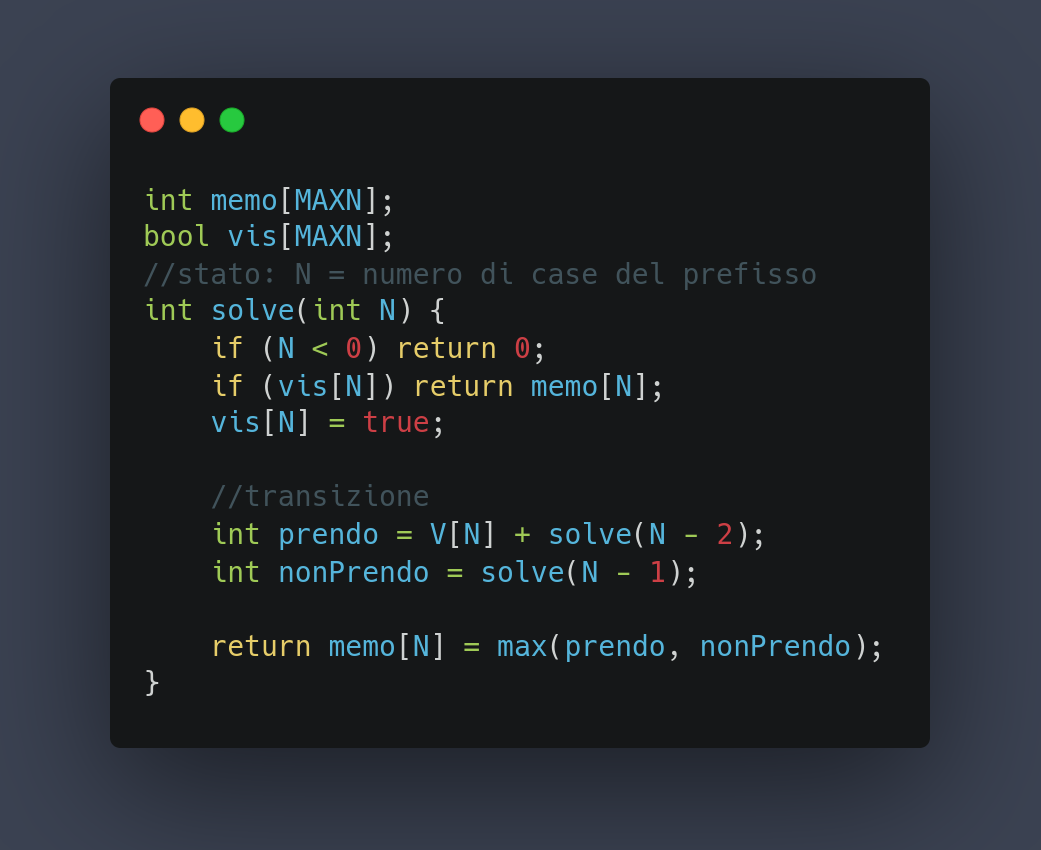
\includegraphics[scale=.25]{./img/hateville_recursive.png}}
\end{frame}

\begin{frame}{Programmazione Dinamica}{Problema: Hateville}
    Riusciamo a risolvere il problema anche in maniera iterativa?
    \pause
    \begin{itemize}
        \item supponiamo di aver processato le prime $i-1$ case.
        \item possiamo trovare la soluzione per le prime $i$ case?
    \end{itemize}
    \pause
    Per ogni $i$, calcoliamo due valori:
    \begin{itemize}
        \item \texttt{prendi[i]}: somma massima considerando le prime $i$ case e prendendo la casa $i$
        \item \texttt{lascia[i]}: somma massima considerando le prime $i$ case e \underline{non} prendendo la casa $i$
    \end{itemize}
\end{frame}
%
\begin{frame}{Programmazione Dinamica}{Problema: Hateville}
    Se stiamo considerando $0$ case, chiaramente \\ \texttt{prendi[0] = lascia[0] = 0}.
    \vfill
    \pause
    Altrimenti
    \begin{itemize}
        \item \texttt{prendi[i] = lascia[i-1] + v[i]}
        \item \texttt{lascia[i] = max(prendi[i-1], lascia[i-1])}
    \end{itemize}
    \vfill
    \pause
    La risposta \`e \texttt{max(prendi[n], lascia[n])}.
    \vfill
    \pause
    La complessit\`a di tempo \`e sempre $O(N)$, anche questa soluzione \`e veloce!
\end{frame}
%
\begin{frame}{Programmazione Dinamica}{Implementazione di Hateville}
    \makebox[\textwidth]{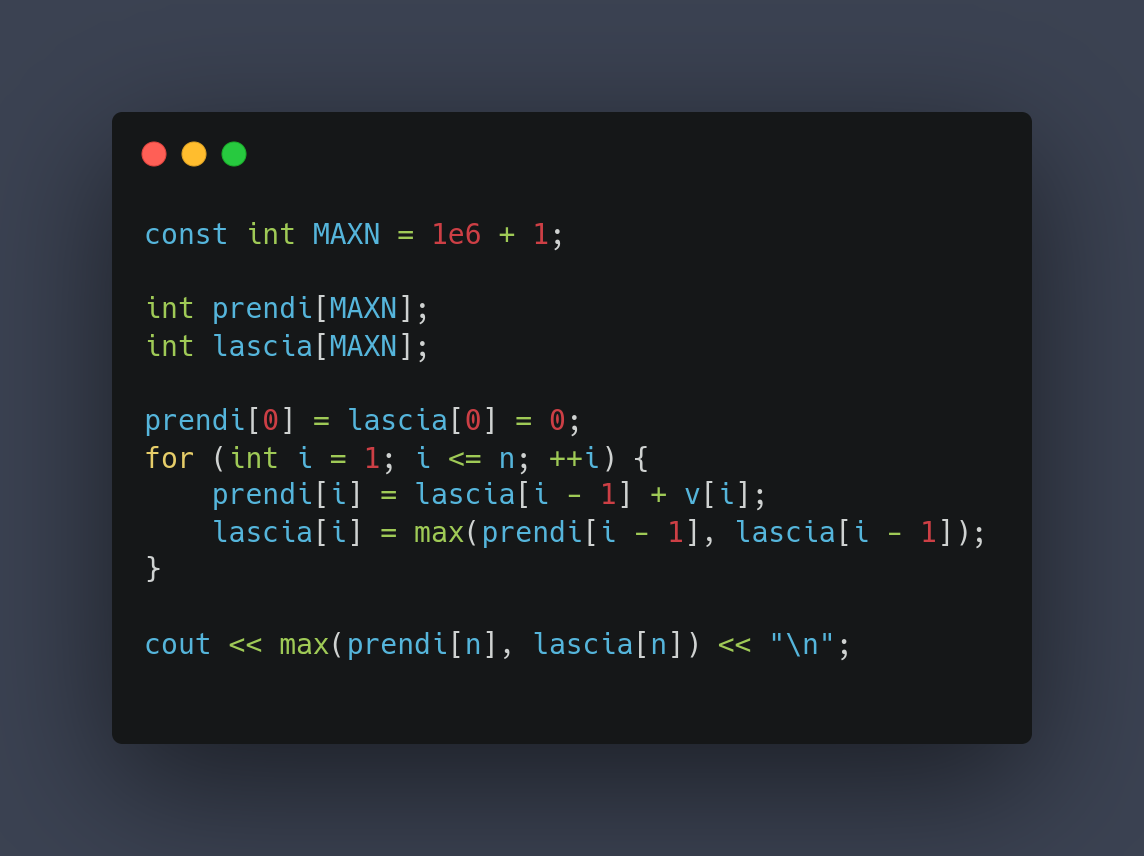
\includegraphics[scale=.25]{./img/hateville_iter.png}}
\end{frame}
%
\begin{frame}{Programmazione Dinamica}{Problema: Frog 1}
    \begin{exampleblock}{Frog 1}
        Ci sono $N$ pietre numerate da $1$ a $N$, ognuna delle quali ha un altezza $h_i$. Una rana \`e inizialmente sulla pietra $1$ e vuole raggiungere la pietra $N$. Se la rana si trova su $i$, pu\`o saltare su $i+1$ o su $i+2$ ad un costo di $|h_i - h_j|$, dove $j$ \`e la pietra su cui atterra. Trova il minimo costo per raggiungere $N$.
    \end{exampleblock}
    \pause
    Anche qui possiamo definire il problema ricorsivamente:
    \[
        dp[i] =
        \begin{cases}
            0 & \text{per } i = N \\
            \begin{split}
                \min(& dp[i+1] + |h_i - h_{i+1}| , \\
                     & dp[i+2] + |h_i - h_{i+2}|)
            \end{split} & \text{per } i < N
        \end{cases}
    \]
    \pause
    \small{\underline{\url{https://atcoder.jp/contests/dp/tasks/dp_a}}}
\end{frame}
%
\begin{frame}{Programmazione Dinamica}{Problema}
    \makebox[\textwidth]{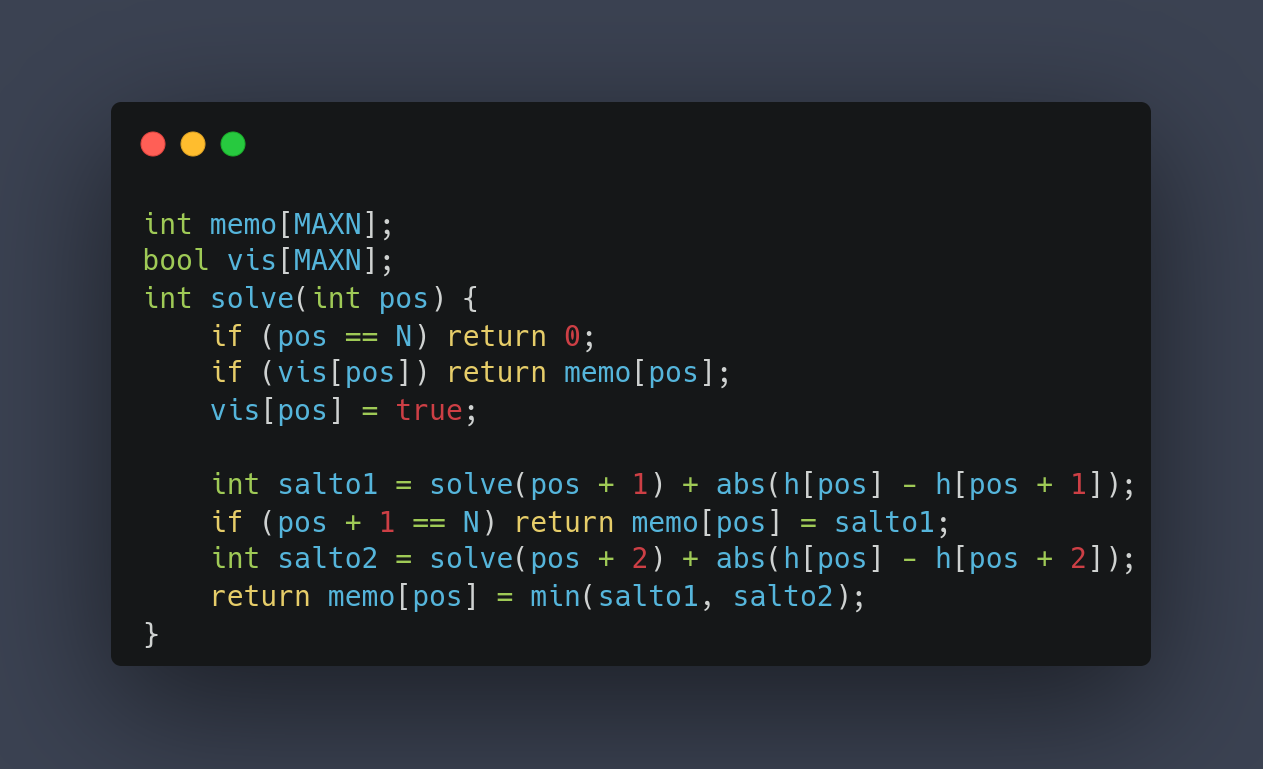
\includegraphics[scale=.25]{./img/frog1.png}}
\end{frame}
%
\begin{frame}{Problemi addizionali}
    %
    \underline{\url{https://training.olinfo.it/\#/task/ois_monopoly/statement}}
    %
    \underline{\url{https://training.olinfo.it/\#/task/preoii_treni/statement}}
    %
    \underline{\url{https://training.olinfo.it/\#/task/luiss_suppli/statement}}
    %
    \underline{\url{https://training.olinfo.it/\#/task/sommelier/statement}}
    %
    \underline{\url{https://training.olinfo.it/\#/task/poldo/statement}}
    %
    \underline{\url{https://training.olinfo.it/\#/task/luiss_laurea/statement}}
    %
\end{frame}
%
\end{document}
